\documentclass[12pt,twoside]{article}
\usepackage[dvipsnames]{xcolor}
\usepackage{tikz,graphicx,amsmath,amsfonts,amscd,amssymb,bm,cite,epsfig,epsf,url}
\usepackage[hang,flushmargin]{footmisc}
\usepackage[colorlinks=true,urlcolor=blue,citecolor=blue]{hyperref}
\usepackage{amsthm,multirow,wasysym,appendix}
\usepackage{array,subcaption} 
% \usepackage[small,bf]{caption}
\usepackage{bbm}
\usepackage{pgfplots}
\usetikzlibrary{spy}
\usepgfplotslibrary{external}
\usepgfplotslibrary{fillbetween}
\usetikzlibrary{arrows,automata}
\usepackage{thmtools}
\usepackage{blkarray} 
\usepackage{textcomp}
\usepackage[left=0.8in,right=1.0in,top=1.0in,bottom=1.0in]{geometry}

\newcommand{\rnd}{\Tilde}
\newcommand{\rx}{\rnd{ x}  }
\newcommand{\ru}{\rnd{ u}  }
\newcommand{\rd}{\rnd{ d}  }
%\newcommand{\rs}{\rnd{ s}  }
\newcommand{\ri}{\rnd{ i}  }
\newcommand{\re}{\rnd{ e}  }
\newcommand{\rQ}{\rnd{ q}  }
\newcommand{\rC}{\rnd{ c}  }
\newcommand{\ra}{\rnd{ a}  }
\newcommand{\rb}{\rnd{ b}  }

\begin{document}


\section*{Bayesian Modelling}
\textbf{Philosophical view}
\begin{enumerate}
    \item Bayesian modelling is different from traditional parametric in a key way, we are trying to model an event, and the parameter used in modelling the event. To do this, we form a prior distribution of our parameter that we believe will be accurate in modelling the underlying event. We observe the event and then our goal is to find the posterior.

    \item the posterior is defined as: f($\theta$  $\vline$ event = event) expanding this, we get 
    
    \begin{equation}
         f(\theta|event = event) = \frac{f(\theta)\times p(Event|\theta)}{P(Event)} 
    \end{equation}

    \item The $\beta$ distribution with parameters a and b is a distribution often used in modelling priors, the pdf takes the form:

    \begin{equation}
    \begin{split}
        f_{a,b} = \frac{t^{a-1}(1-t)^{b-1}}{\beta(a,b)} \\
         \text{where } \beta = \int_u^\infty u^{a-1}(1-u)^{b-1}du
    \end{split}
    \end{equation}
    
    \item Lastly, the $\beta$ distribution is a conjugate prior, meaning if we use a $\beta$ distribution to model the prior of our parameter, the posterior will also be a $\beta$ distribution with a different parameter which is mathematically convenient. 
\end{enumerate}
    
\section*{Expectation and Variance of Random Variables}
\textbf{Expectation:}
The expectation or mean of a random variable $\ra$ is equal to:
$$
    E(\ra) = \frac{1}{n} \times \sum_{i=1}^n \ra_i p_{\ra}(\ra = \ra_i)
$$
\textbf{Linearity of Expectation:}
The expectation or mean of the sum of two random variable $\ra$ and $\rb$ is equal to:
$$
    E(\ra+\rb) = E(\ra)+E(\rb)
$$
\textbf{Mean of scaled Random Variables:}
The expectation or mean of a scaled random variable $\alpha\ra$ is equal to:
$$
    E(\alpha\ra) = \alpha E(\ra)
$$
\textbf{Multiplication of Random Variables:}\\
If two random variables, $\ra$ and $\rb$ come from the same distribution and are independent then the following equality holds:
$$
    E(\ra \rb) = E^2(\ra) = E^2(\rb) = E(\ra)E(\rb)
$$
\textbf{Variance:}
The variance of a random variable $\ra$ is equal to:
$$
    Var(\ra) = E((\ra-\mu_{\ra})^2) = \frac{1}{n} \times \sum_{i=1}^n (\ra_i-\mu_{\ra})^2 
$$
We can use a shortcut to express the variance in a simplified form:
\begin{equation}
    \begin{split}
        Var(\ra) &= E((\ra-\mu_{\ra})^2) \\
        &= E(\ra^2 - 2\mu_{\ra}\ra + \mu_{\ra}^2) \\
        &= E(\ra^2) - \mu_{\ra}E(2\ra + \mu_{\ra}) \\   
        &= E(\ra^2) - 2\mu_{\ra}^2 + \mu_{\ra}^2 \\ 
        &= E(\ra^2) - E^2(\ra)
    \end{split}
\end{equation}
\textbf{Variance of the sum of two random variables:}
\begin{equation}
    \begin{split}
        Var(\ra+\rb) &= E((\ra+\rb-E(\ra+\rb))^2) \\
        &= E((\ra+\rb-\mu{\ra}-\mu_{\rb}))^2) \\
        &= E((\ra-\mu_{\ra})^2) + E((\rb-\mu_{\rb})^2) + 2E((\ra-\mu_{\ra})(\rb - \mu{\rb})) \\   
        &= Var(\ra) + Var(\rb) +2Cov(\ra,\rb) 
    \end{split}
\end{equation}
If the two random variables are uncorrelated then:
$$
    Var(\ra+\rb) = Var(\ra) + Var(\rb)
$$
\section*{PDF, PMF Mean and Variance of Popular Distributions:}
\textbf{Binomial:} 
$$Mean = n\theta \qquad Variance = n\theta(1-\theta) \qquad PMF = \begin{pmatrix} n \\ k \end{pmatrix} \theta^k(1-\theta)^{n-k}$$
\textbf{Bernoulli:} 
$$Mean = \theta \qquad Variance = \theta(1-\theta) \qquad PMF = \begin{cases} \theta & if k=1 \\ 1-\theta & if \ k=0 \end{cases}$$
\textbf{Geometric:} 
$$Mean = \frac{1}{\theta} \qquad Mean \ Squared = E(\rx^2) = \frac{2-\theta}{\theta^2} \qquad Variance = \frac{1-\theta}{\theta^2} \qquad PMF = (1-\theta)^{k-1}\theta$$
\textbf{Exponential:} 
$$Mean = E(\rx) = \frac{1}{\lambda} \qquad Mean \ Squared = E(\rx^2) = \frac{2}{\lambda^2}\qquad Variance = \frac{1}{\lambda^2} \qquad PMF = \lambda e^{-\lambda t}$$
\textbf{Poisson:} 
$$Mean = E(\rx) = \lambda \qquad Mean \ Squared = E(x^2) = \lambda + \lambda^2 \qquad Variance = \lambda \qquad PMF = (1-\theta)^{k-1}\theta$$
\textbf{Gaussian:} 
$$Mean = \mu \qquad Variance = \sigma^2$$
\textbf{Uniform:} 
$$Mean = \frac{a+b}{2} \qquad Variance = \frac{(b-a)^2}{12} \qquad PDF = \frac{1}{b-a}$$
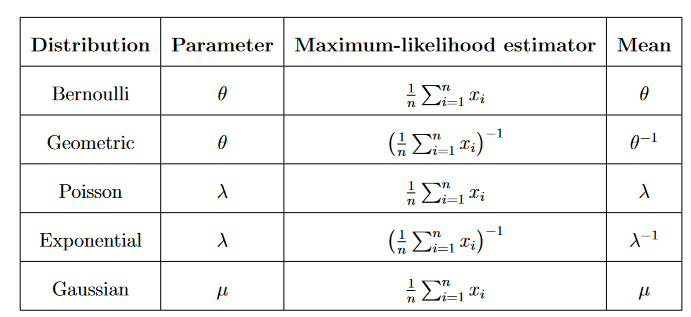
\includegraphics[scale=.8]{mean of distributions.png}

\section*{Joint, Marginal, and Conditional Distributions}
\textbf{Joint}

\textbf{Marginal} If you want the marginal of x, you sum over y
\textbf{Conditional} $$
    Conditional = \frac{joint}{marginal}
$$

\newpage 
\section*{Standardized Random Variables and Linear Estimation}
\textbf{Standardizing a Random Variable}:
How to standardize a random variable, $\ra$, such that its mean centered and unit variance:
$$
    s(a) = \frac{\ra-\mu_{\ra}}{\sigma_{\ra}}
$$
\textbf{Linear Estimates:}
Best linear estimate of b given a is correlation coefficient times a equals b estimate (plus error):
$$
    \hat{b} = \mu_{\rb} + \sigma_{\rb} \times \rho_{\ra,\rb} \times s(\ra)
$$
Remember, if $\ra$ isn't standardized, make sure to standardize it. For hw/test problems, start by defining what you're predicting, and what the predictor is, then calculate the expectation, variance, and std. dev of your predictor, the cov and corr of the predictor/predicion, then fill in formula.\\
If our random variables $\ra$ and $\rb$ are standardized, the linear estimate is expressed in the following way:
$$
    \hat{b} = \rho_{\ra,\rb} \times s(\ra)
$$
Which makes sense as $$E(\rb)=0 \text{ and } Var(\rb)=1$$
\section*{Co-Variance and Correlation}
\textbf{Covariance:}
We define the co-variance of $\ra$ and $\rb$:
$$
Cov(\ra , \rb) = E((\ra-\mu_{\ra})(\rb - \mu{\rb}))
$$
We can use a shortcut to express the co-variance in a simplified form:
\begin{equation}
    \begin{split}
       Cov(\ra , \rb) &= E((\ra-\mu_{\ra})(\rb - \mu{\rb})) \\
       &= E(\ra \rb) - \mu_{\rb}E(\ra) - \mu_{\ra}E(\rb) +\mu_{\ra}\mu_{\rb}\\
       &= E(\ra \rb) - \mu_{\ra}\mu_{\rb} - \mu_{\ra}\mu_{\rb} +\mu_{\ra}\mu_{\rb}\\
       &= E(\ra \rb) - \mu_{\ra}\mu_{\rb} 
    \end{split}
\end{equation}
If our random variables $\ra$ and $\rb$ are standardized, correlation is expressed the following way:
$$
Cov(\ra , \rb) =  E(\ra \rb)
$$   
Which makes sense as: $$E(\ra) = E(\rb) = 0$$
\textbf{Correlation:}
The correlation between two random variables $\ra$ and $\rb$ is defined as:
$$
    Corr(\ra,\rb) = \rho_{\ra,\rb} = \frac{Cov(\ra,\rb)}{\sigma_{\ra} \times \sigma_{\rb}}
$$
If the random variables are mean centered and standardized then the correlation is the same as co-variance:
$$
Corr(\ra,\rb) = \rho_{\ra,\rb} = Cov(\ra,\rb)
$$
Which makes sense as $$\sigma_{\ra}^2=0 \text{ and } \sigma_{\rb}^2=0$$
\textbf{Mean Squared Error of MMSE Estimate:}
The linear MMSE estimate of $\rb$ given $\ra$ is:
$$
    E((\alpha \times \ra + \beta -\rb)^2) = (1-\rho_{\ra,\rb}^2) \times \sigma_{\rb}^2
$$
\textbf{Consequences of the MMSE Estimate:}
\begin{enumerate}
    \item correlation coefficient is bounded between -1 and 1.
    \item When it equals -1 or 1, it implies a linear relationship between the random variables $\ra$ and $\rb$
    \item The square of the correlation coefficient is the fraction of variance in $\rb$ that can be explained linearly in terms of $\ra$
\end{enumerate}
\section*{Main Takeaways}
\textbf{Facts about correlation, expectation, co-variance, and standardized random variables:}
\begin{enumerate}
    \item If your random variables are mean centered and standardized, then the mean is 0 and the variance is 1. The variance will also equal the expectation of your random variable squared. 
    \subitem Expectation $\rightarrow E(\ra) = 0$ Variance $\rightarrow E(\ra^2)=1$
    \item If you have two (or more) random variables that are mean-centered and standardized, the correlation equals to covariance 
    \subitem Cov($\ra,\rb$)=Corr($\ra,\rb$)
    \item Linear Estimate residuals have an expectation of 0
    \subitem $E(\rb - (\mu_{\rb} + \sigma_{\rb} \times s(\ra)))=0$
    \item Linear Estimates and residuals have 0 co-variance, and are uncorrelated
    \item Two random variables that are independent implies that they are also uncorrelated. Surprisingly, the opposite is not true. Two random variables being uncorrelated does not mean they are independent.  
    
\end{enumerate}

\section*{Problem Solving Strategies}
\textbf{Inverse Sampling}
\begin{enumerate}
    \item Step 1: Determine whether the problem is asking you to find the X that would result in a uniform distribution value, or find the x that would give you the supplied uniform distribution.
    
    \item Case 1: In the case you're given a uniform distribution value, and want to find the corresponding x.
    \subitem calculate the CDF of the function
    \subitem Swap the x and y in the CDF and solve for y again, obtaining the inverse cdf
    \subitem If your CDF consists of multiple functions depending on the value of x, determine which inverse CDF you should use by looking at the given value of the uniform distribution sample. 
    \subitem plug in the uniform value as x into the proper inverse cdf, solving for y
    
    \item Case 2: If you are given an x value and trying to get the corresponding uniform value.
    \subitem plug x into the appropriate CDF and you will get a value in the 0-1 domain 
  
\end{enumerate}

\section*{Markov’s Inequality}
Let $\ra$ be a non-negative random variable. For any positive
constant $c > 0$
\begin {equation}
     P (\ra \geq c) \leq \frac{E(\ra)}{c}
    \end {equation} 
    
\section*{Chebyshev's Inequality}
For any positive constant $c > 0$ and any random variable $\ra$ with bounded variance:
\begin{equation}
    P((\ra - E(\ra) \geq c)) \leq \frac{Var(\ra)}{c}
\end{equation}
\section*{Chebyshev Continued}
Probability that the sample mean deviates from the population mean by more than c (Where n is sample size).
\begin {equation} 
    P( x\Bar{}-\mu > c)= \frac{\sigma^2}{nc^2}
    \end {equation}
    Step 1: If you don't know the variance, make a reasonable estimate of the upper bound. \\
    Step 2: If you're given a bound with respect to distance for your confidence interval,(i.e. we want to have a 95\% confidence interval that does not exceed 5cm), you'll have to divide the distance (width) by 2, and put that value into Chevysevs.\\ 
    Step 3: Do the following computation:
    $$
      P( x\Bar{}-\mu > c)= 1 - \alpha =  \frac{\sigma^2}{n(\frac{c}{2})^2}  
    $$
    Step 4: The answer from the computation gives us the minimum sample size we need to guarantee a confidence interval of a certain width.
    

\section*{Confidence Interval}
Take the mean, and get your bounds by adding (for top bound) and subtracting (for lower bound) the following expression:
$$
   Upper \  Bound = \mu + \frac{\sigma}{\sqrt{n}} \times \text{z-score} \qquad Lower \ Bound = \mu - \frac{\sigma}{\sqrt{n}} \times \text{z-score}
$$
\textbf{Popular Z Scores:}
$$
\begin{pmatrix}
Confidence Level & Area \  between \  0 \ and \ z-score & z-score \\
90\%	& 0.4500	& 1.645 \\
95\%	& 0.4750	& 1.960 \\
98\%	& 0.4900	& 2.326 \\
99\%	& 0.4950	& 2.576 \\
\end{pmatrix}$$

\section*{Miscellaneous}
\textbf{Gaussian vectors}
\begin{enumerate}
    \item A Gaussian vectors x in ${R^d}$ has co-variance matrix ${x^Tx}$. 
    \item The probability density of Gaussian vector x is defined as ${x^T}$ $\Sigma{^-1}$x where $\Sigma$ is the inverse of the co-variance matrix.
    \item Any linear transformation of a Gaussian vector results in a Gaussian vector, so the equation:
    \subitem As a result the following is a Gaussian vector where A is an ${R^mxd}$ matrix
        \begin{equation}
             y = Ax + b 
        \end{equation}
    \item Additionally the marginal and conditional distributions of Gaussian vectors are Gaussian vectors
    \subitem the density of the marginal distribution is 
       \begin{equation}
             f(a) = (1/\sqrt{2\pi}) \times \exp{\frac{-a^2}{2}}
        \end{equation}
    \subitem The conditional density is given by:
      \begin{equation}
             f(b|a) = (1/\sqrt{2\pi\times(1-\rho^2}) \times \exp{\frac{(b-\rho\times a)^2}{2\times(1-\rho^2)}}
        \end{equation}
    \subitem Lastly the mean and variance of a gaussian vector b given a is:
        \begin{equation}
            \mu_{b|a} = \mu_b \frac{\rho\sigma_b(a-\mu_a}{\sigma_b}
        \end{equation}
        \begin{equation}
             \sigma^2_{b|a} = (1-\rho^2)\sigma^2_b
        \end{equation}

\end{enumerate}

Proof: Final Exam Study Question 5
$$Var(n\tilde{x}+\sum_{i=1}^{n}\tilde{z}_{i})$$

$$= Var(n\tilde{x} +n\cdot \frac{1}{n}\sum_{i=1}^{n}\tilde{z}_{i})$$

$$= Var(n(\tilde{x} +\frac{1}{n}\sum_{i=1}^{n}\tilde{z}_{i}))$$

$$ = n^{2} Var(\tilde{x} +\frac{1}{n}\sum_{i=1}^{n}\tilde{z}_{i})$$

$$= n^{2} (Var(\tilde{x}) + Var(\frac{1}{n}\sum_{i=1}^{n}\tilde{z}_{i}))$$  given x and z are independent

$$= n^{2} (1+\frac{\sigma ^{2}}{n})$$

$$= n^{2} +n{\sigma ^{2}}$$




$$Var(\frac{1}{n}\sum_{i=1}^{n}\tilde{z}_{i})$$

$$=\frac{1}{n^{2}}Var(\sum_{i=1}^{n}\tilde{z}_{i})$$

$$=\frac{1}{n^{2}}n\sigma ^{2}$$

$$=\frac{\sigma ^{2}}{n}$$
\end{document}
